\documentclass[11pt,letterpaper]{article}
\input{glyphtounicode}
\pdfgentounicode=1
\usepackage[utf8]{inputenc}
\usepackage[T1]{fontenc}
\usepackage{lmodern}
\usepackage[spanish,es-noindentfirst,es-tabla]{babel}
\decimalpoint
\usepackage[margin=2.5cm]{geometry}
\usepackage{graphicx}
\usepackage{booktabs}
\usepackage{array}
\usepackage{multirow}
\usepackage{siunitx}
\sisetup{output-decimal-marker={.}, group-digits=false, detect-weight=true, table-number-alignment=center}
\usepackage{amsmath,amssymb}
\usepackage{listings}
\renewcommand{\lstlistingname}{Código}
\usepackage{xcolor}
\usepackage{tikz}
\usetikzlibrary{positioning,arrows.meta,shapes.geometric}
\usepackage{fancyhdr}
\usepackage{titlesec}
\usepackage{caption}
\usepackage[section]{placeins}
\usepackage[hidelinks]{hyperref}
\graphicspath{{figuras/}}
\renewcommand{\topfraction}{0.92}
\renewcommand{\bottomfraction}{0.85}
\renewcommand{\textfraction}{0.06}
\renewcommand{\floatpagefraction}{0.80}
\setcounter{topnumber}{3}
\setcounter{totalnumber}{5}
\captionsetup{font=small,labelfont=bf,textfont=it,labelsep=newline,justification=raggedright,singlelinecheck=false,skip=4pt}
\newcommand{\nota}[1]{\par\vspace{2pt}{\footnotesize\raggedright\textit{Nota.} #1\par}}

\lstdefinestyle{codigo}{
    language=Python,
    basicstyle=\ttfamily\footnotesize,
    keywordstyle=\color{blue!60!black}\bfseries,
    commentstyle=\color{gray},
    stringstyle=\color{orange!70!black},
    numbers=left,
    numberstyle=\tiny\color{gray},
    frame=single,
    breaklines=true,
    showstringspaces=false,
    tabsize=4,
    backgroundcolor=\color{gray!5},
    extendedchars=true,
    columns=fullflexible,
    keepspaces=true,
    literate={á}{{\'a}}1 {é}{{\'e}}1 {í}{{\'i}}1 {ó}{{\'o}}1 {ú}{{\'u}}1
             {Á}{{\'A}}1 {É}{{\'E}}1 {Í}{{\'I}}1 {Ó}{{\'O}}1 {Ú}{{\'U}}1
             {ñ}{{\~n}}1 {Ñ}{{\~N}}1 {¿}{{?`}}1 {¡}{{!`}}1 {±}{{$\pm$}}1
}
\lstset{style=codigo}

\pagestyle{fancy}
\fancyhf{}
\rhead{Inteligencia Computacional Aplicada}
\cfoot{\thepage}
\renewcommand{\headrulewidth}{0.4pt}
\titleformat{\section}{\normalfont\Large\bfseries}{\thesection.}{0.5em}{}
\titleformat{\subsection}{\normalfont\large\bfseries}{\thesubsection}{0.5em}{}

\newcommand{\nombreEstudiante}{Sergio Santiago Duarte Rojas}
\newcommand{\codigoEstudiante}{20261595002}
\newcommand{\nombreDocente}{Cesar Andrey Perdomo Charry}
\newcommand{\nombreAsignatura}{Inteligencia Computacional Aplicada}


\usepackage{xurl}
\newcommand{\difSemMedia}{1.11}
\newcommand{\difSemDesv}{0.49}
\newcommand{\nSemSig}{4}
\newcommand{\sigBase}{33.0}
\newcommand{\sigUno}{24.5}
\newcommand{\sigSeis}{57.7}
\newcommand{\sigCuad}{9.7}
\newcommand{\aicBase}{4854.9}
\newcommand{\aicCuad}{3930.9}
\newcommand{\kapCuad}{0.347}
\newcommand{\sesgoBase}{0.72}
\newcommand{\sesgoSin}{3.58}
\newcommand{\sesgoNarSin}{2.03}
\newcommand{\epSin}{87}
\newcommand{\pBase}{229}
\newcommand{\epSesentaCero}{261}
\newcommand{\trSesentaCero}{0.038}
\newcommand{\vaSesentaCero}{0.147}
\newcommand{\parSesentaCero}{1217}
\newcommand{\epDosCapasCero}{216}
\newcommand{\trDosCapasCero}{0.040}
\newcommand{\vaDosCapasCero}{0.159}
\newcommand{\parDosCapasCero}{1121}
\newcommand{\epCuatroL}{600}
\newcommand{\trCuatroL}{0.120}
\newcommand{\vaCuatroL}{0.165}
\newcommand{\parCuatroL}{77}
\newcommand{\epBase}{450}
\newcommand{\trBase}{0.074}
\newcommand{\vaBase}{0.139}
\newcommand{\parBase}{229}

\hypersetup{pdftitle={Series de tiempo. Taller 1, métodos clásicos frente a redes NAR y NARX}, pdfauthor={Sergio Santiago Duarte Rojas}}
\lhead{Series de tiempo, Taller 1}

\begin{document}

\begin{titlepage}
    \centering
    \vspace*{2cm}
    {\LARGE \bfseries Series de tiempo. Taller 1\\[4pt] Métodos estadísticos clásicos frente a redes neuronales NAR y NARX\par}
    \vspace{0.5cm}
    {\large Informe\par}
    \vspace{2cm}
    \begin{tabular}{ll}
        \textbf{Asignatura:} & \nombreAsignatura \\
        \textbf{Docente:}    & \nombreDocente \\
        \textbf{Estudiante:} & \nombreEstudiante \\
        \textbf{Código:}     & \codigoEstudiante \\
        \textbf{Fecha:}      & 3 de noviembre de 2026 \\
    \end{tabular}
    \vfill
    Universidad Distrital Francisco José de Caldas
\end{titlepage}

\tableofcontents
\newpage

\section{Introducción}

Los siete experimentos de la sección 11 del cuaderno se evaluaron sobre una misma configuración base. La ventaja de NARX sobre SARIMAX depende de la fracción de la demanda que corresponde a la no linealidad de la temperatura. Desaparece cuando SARIMAX recibe el término cuadrático o cuando el proceso es lineal, y se invierte cuando el ruido domina la señal. Dentro de la red, el desempeño depende de que la ventana de retardos cubra el periodo estacional, de que la capacidad sea moderada y de que la tendencia se retire antes del entrenamiento. A un paso, NARX supera a SARIMAX en las seis semillas evaluadas con la configuración base, con diferencia significativa en \nSemSig{} de ellas.

\section{Marco teórico (resumen)}

La demanda sigue un proceso generador conocido con tendencia lineal, estacionalidad semanal ($S=7$), el término $\kappa\,(x_t-18)^2$ con $\kappa=0.35$, el efecto retardado $3\tanh(x_{t-1}-20)$ y un ruido AR(1) con innovaciones de varianza $\sigma^2$. SARIMAX es lineal en sus regresores exógenos (Box et al., 2015), de modo que la componente cuadrática no representada se traslada al error. NARX aproxima la relación entre los retardos de la salida y de la exógena con una red neuronal, sin una forma funcional especificada (Leontaritis y Billings, 1985). Su error de generalización combina sesgo, que se reduce con la capacidad, y varianza, que crece con ella y se controla con regularización $L_2$ y parada temprana. La activación $\tanh$ es acotada, por lo que la red no extrapola niveles fuera del rango de entrenamiento.

La comparación entre modelos emplea la prueba de Diebold y Mariano (1995) con la corrección de Harvey et al. (1997). Con pérdida cuadrática, un estadístico positivo favorece al segundo modelo del par. La prueba de Ljung y Box (1978) evalúa la autocorrelación remanente en los residuos.

\section{Metodología}

La configuración base es la del cuaderno del curso con la semilla 43, esto es, SARIMAX de órdenes $(2,0,1)$ y $(1,1,1)_7$ con $x_t$ como exógena y redes de una capa oculta de 12 neuronas, 14 retardos de la salida ($d_y$), 3 de la exógena, $L_2=10^{-4}$ y tendencia retirada. La partición temporal asigna 766 días al entrenamiento, 164 a la validación y 165 a la prueba. Cada experimento modifica un único elemento de la base (Tabla~\ref{tab:diseno}). Los modelos clásicos se ajustan con statsmodels (Seabold y Perktold, 2010) y las redes con TensorFlow. La semilla determina la realización de la serie y la inicialización de las redes, de modo que los experimentos 1 a 6 comparten los datos de la base y el experimento 7 varía ambos.

\begin{table}[!htb]
    \centering
    \caption{Diseño de los experimentos}
    \label{tab:diseno}
    \footnotesize
    \begin{tabular}{c l l}
        \toprule
        \textbf{Subgrupo} & \textbf{Variación respecto a la base} & \textbf{Pregunta} \\
        \midrule
        1 & SARIMAX recibe $x_t$ y $(x_t-18)^2$ & reducción de la diferencia con NARX \\
        2 & $\kappa=0$, proceso lineal en $x_t$ & desempeño de la red y parsimonia \\
        3 & $d_y\in\{3,7,14,28\}$ & error a uno y a 14 pasos \\
        4 & neuronas $\in\{[4],[12],[64],[32,16]\}$, $L_2\in\{0,10^{-3}\}$ & sesgo y varianza \\
        5 & $\sigma\in\{1,3,6\}$ & ventaja de la red con más ruido \\
        6 & sin retirar la tendencia & extrapolación con $\tanh$ \\
        7 & semillas 1 a 5 & estabilidad de la diferencia \\
        \bottomrule
    \end{tabular}
\end{table}

\section{Resultados}

La Tabla~\ref{tab:general} reúne la raíz del error cuadrático medio en prueba de los tres modelos de interés y la prueba de Diebold y Mariano entre SARIMAX y NARX para cada configuración. Holt-Winters y el ingenuo estacional no dependen de las variaciones de los subgrupos 1, 3, 4 y 6.

\begin{table}[!htb]
    \centering
    \caption{Raíz del error cuadrático medio en prueba y prueba de Diebold y Mariano entre SARIMAX y NARX a un paso}
    \label{tab:general}
    \scriptsize
    \setlength{\tabcolsep}{4.5pt}
    \begin{tabular}{c l c c c c c c c}
        \toprule
        & & \multicolumn{3}{c}{\textbf{A un paso}} & \multicolumn{2}{c}{\textbf{A 14 pasos}} & \multicolumn{2}{c}{\textbf{Diebold y Mariano}} \\
        \cmidrule(lr){3-5}\cmidrule(lr){6-7}\cmidrule(lr){8-9}
        \textbf{Subgrupo} & \textbf{Configuración} & SARIMAX & NARX & NAR & SARIMAX & NARX & DM* & $p$ \\
        \midrule
\csname @@input\endcsname tabla_experimentos.tex
        \bottomrule
    \end{tabular}
    \nota{Un estadístico DM* positivo favorece a NARX y uno negativo a SARIMAX. La base usa [12] neuronas con $\lambda=10^{-4}$ y $d_y=14$.}
\end{table}

\begin{figure}[!htb]
    \centering
    \caption{Error en prueba frente a los retardos de la salida (izquierda) y frente al nivel de ruido (derecha)}
    \label{fig:retardos}
    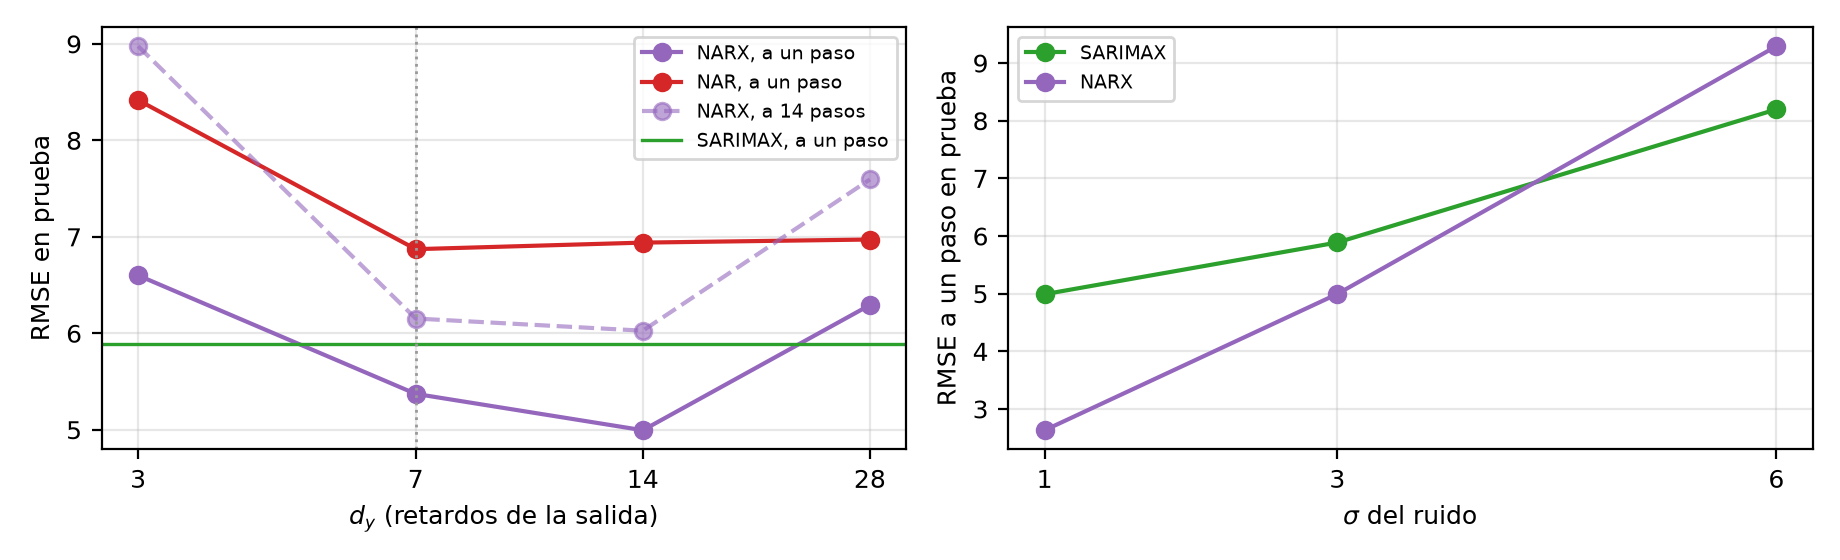
\includegraphics[width=15.5cm]{fig01_retardos_ruido.png}
    \nota{La línea punteada vertical marca el periodo estacional $S=7$. Verde SARIMAX, morado NARX y rojo NAR, la misma asignación del cuaderno.}
\end{figure}

\begin{figure}[!htb]
    \centering
    \caption{Curvas de aprendizaje de NARX según la capacidad y la regularización}
    \label{fig:curvas}
    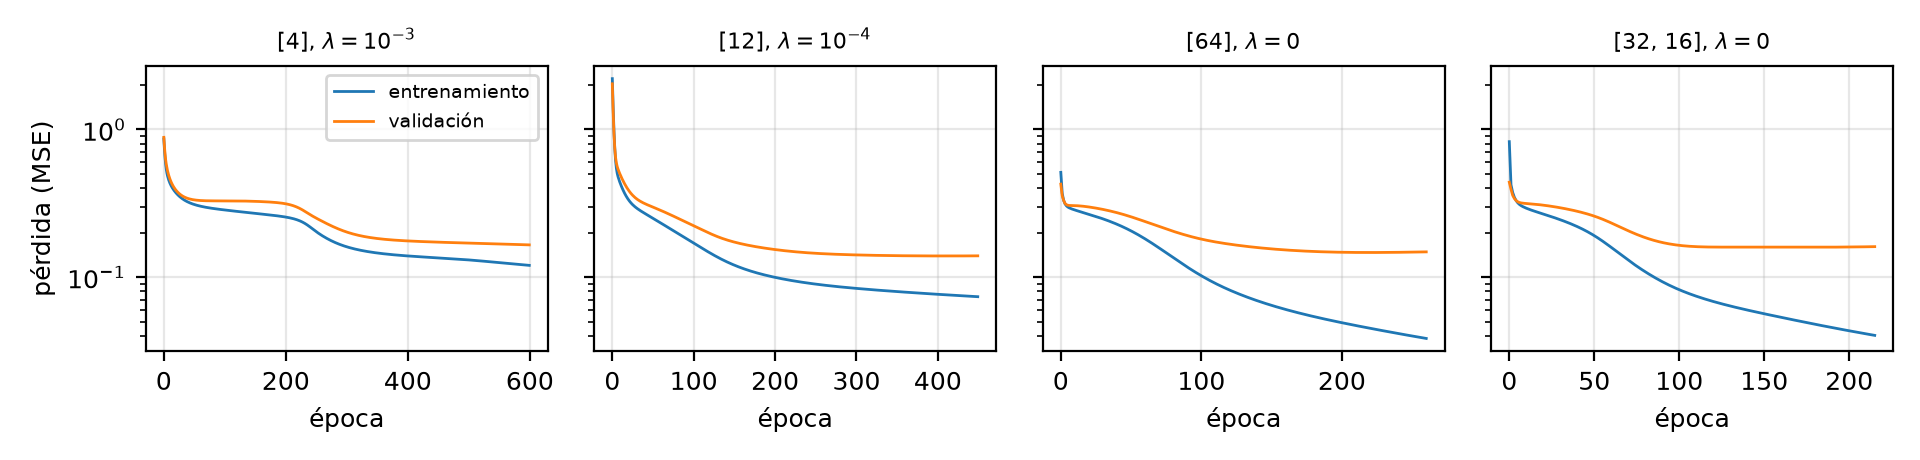
\includegraphics[width=15.5cm]{fig02_curvas_aprendizaje.png}
    \nota{Pérdida del mejor de los tres reinicios, en escala logarítmica. Azul entrenamiento y naranja validación.}
\end{figure}

\section{Análisis}

\subsection{Subgrupo 1, ingeniería de variables}

Con $(x_t-18)^2$ como regresor, SARIMAX estima $\kappa$ en \kapCuad, con intervalo de 95~\% entre 0.330 y 0.363, y su varianza de innovación desciende de \sigBase{} a \sigCuad, próxima a la varianza 9 del ruido. El criterio de Akaike disminuye de \aicBase{} a \aicCuad. La diferencia con NARX se invierte y Diebold y Mariano resulta significativo a favor de SARIMAX, que emplea 9 parámetros frente a \pBase. La ventaja de la red en la base correspondía a una no linealidad de forma conocida, ausente de los regresores lineales.

\subsection{Subgrupo 2, proceso lineal}

Con $\kappa=0$, SARIMAX supera a NARX a uno y a 14 pasos ($p=0.018$), y NAR y NARX no difieren entre sí ($p=0.70$), porque la exógena solo conserva el efecto retardado. Su varianza de innovación es la misma que con el término cuadrático, lo que indica que en ambos casos la parte lineal del modelo cubre toda la estructura disponible. Por parsimonia corresponde elegir SARIMAX.

\subsection{Subgrupo 3, retardos de la salida}

El error de NARX es mínimo con $d_y=14$, el doble del periodo estacional (Figura~\ref{fig:retardos}). Con $d_y=3$ la ventana no alcanza el retardo 7, donde la función de autocorrelación parcial de la serie diferenciada concentra la dependencia estacional, y el error a 14 pasos sube de 6.03 a 8.98, porque en lazo cerrado el ciclo semanal debe reconstruirse con predicciones propias. Con $d_y=28$ la red alcanza la menor pérdida de entrenamiento de las cuatro ventanas, pero no la menor de validación, y sus residuos conservan autocorrelación ($p<0.001$ en Ljung y Box). La ventana debe cubrir al menos un periodo estacional y su ampliación posterior agrega varianza.

\subsection{Subgrupo 4, capacidad y regularización}

Las redes grandes sin regularización muestran sobreajuste en las curvas de aprendizaje (Figura~\ref{fig:curvas}). Con [64] neuronas y $\lambda=0$ la parada temprana actúa en la época \epSesentaCero, con pérdida de entrenamiento de \trSesentaCero{} y de validación de \vaSesentaCero, cerca de cuatro veces mayor. Con [32, 16] la relación es similar desde la época \epDosCapasCero. La regularización $\lambda=10^{-3}$ reduce el error de prueba de las dos arquitecturas grandes. Con [4] neuronas y $\lambda=10^{-3}$ las curvas se mantienen próximas hasta la época \epCuatroL{} (\trCuatroL{} frente a \vaCuatroL), y esa configuración obtiene el menor error a uno y a 14 pasos del subgrupo, con \parCuatroL{} parámetros. Para 766 días de entrenamiento, la capacidad necesaria es baja.

\subsection{Subgrupo 5, relación señal a ruido}

La ventaja de NARX disminuye al aumentar el ruido y se invierte con $\sigma=6$ (Figura~\ref{fig:retardos}). La varianza de innovación de SARIMAX es \sigUno, \sigBase{} y \sigSeis{} para $\sigma$ de 1, 3 y 6, y al restar la varianza del ruido queda en todos los casos un remanente de 22 a 24, que corresponde a la componente no lineal no representada. Esa componente explica cerca del 96~\% de la varianza de innovación con $\sigma=1$, el 73~\% con $\sigma=3$ y el 38~\% con $\sigma=6$. Cuando la no linealidad es una fracción menor de la variabilidad, lo que la red gana al modelarla es inferior a la varianza que agregan sus 229 parámetros.

\subsection{Subgrupo 6, tendencia sin retirar}

Sin retirar la tendencia, el error medio de NARX en prueba pasa de \sesgoBase{} a \sesgoSin, y el de NAR de 0.35 a \sesgoNarSin. El signo positivo indica predicciones sistemáticamente inferiores a los valores observados. La tendencia de 0.03 por día lleva la demanda de prueba por encima del rango de entrenamiento, y la salida de las neuronas $\tanh$, acotada, no alcanza esos niveles. La parada temprana actúa en la época \epSin{} y el error a un paso sube de 5.00 a 8.38. SARIMAX no se ve afectado, porque la diferenciación estacional absorbe la tendencia.

\subsection{Subgrupo 7, variabilidad entre semillas}

A un paso, NARX supera a SARIMAX en las seis semillas, con una diferencia media de \difSemMedia{} en la raíz del error cuadrático medio (desviación \difSemDesv) y diferencia significativa en \nSemSig{} de ellas. A 14 pasos el orden se mantiene solo en tres semillas, de modo que la ventaja a un paso es estable en signo y la ventaja en lazo cerrado depende de la realización.

\section{Conclusiones}

La ventaja de NARX sobre SARIMAX en este proceso proviene de una sola no linealidad. Cuando esa forma se incorpora como regresor o no está presente, el modelo lineal es más preciso y más parsimonioso, y cuando el ruido domina, la varianza de la red supera lo que gana al modelarla (Tabla~\ref{tab:general}).

El desempeño de la red exige decisiones de diseño ligadas a la serie. La ventana de retardos debe cubrir el periodo estacional, la capacidad debe ser baja frente al tamaño del entrenamiento y la tendencia debe retirarse, porque la activación $\tanh$ no extrapola. Con esas condiciones, su ventaja a un paso se mantiene entre semillas.

\section{Declaración de uso de inteligencia artificial}

Se usó Claude como apoyo en la redacción, la revisión de consistencia entre conceptos y la preparación de tablas y gráficas. Los procedimientos, las modificaciones al código fuente y la estructura del documento son del autor, quien verificó cada cifra con las salidas del cuaderno.

\section{Referencias}

\begin{itemize}
    \setlength{\itemsep}{2pt}
    \item[] Box, G. E. P., Jenkins, G. M., Reinsel, G. C., \& Ljung, G. M. (2015). \textit{Time series analysis: Forecasting and control} (5.ª ed.). Wiley.
    \item[] Diebold, F. X., \& Mariano, R. S. (1995). Comparing predictive accuracy. \textit{Journal of Business \& Economic Statistics, 13}(3), 253--263. \url{https://doi.org/10.1080/07350015.1995.10524599}
    \item[] Harvey, D., Leybourne, S., \& Newbold, P. (1997). Testing the equality of prediction mean squared errors. \textit{International Journal of Forecasting, 13}(2), 281--291. \url{https://doi.org/10.1016/S0169-2070(96)00719-4}
    \item[] Leontaritis, I. J., \& Billings, S. A. (1985). Input-output parametric models for non-linear systems Part I: Deterministic non-linear systems. \textit{International Journal of Control, 41}(2), 303--328. \url{https://doi.org/10.1080/00207178508961129}
    \item[] Ljung, G. M., \& Box, G. E. P. (1978). On a measure of lack of fit in time series models. \textit{Biometrika, 65}(2), 297--303. \url{https://doi.org/10.1093/biomet/65.2.297}
    \item[] Seabold, S., \& Perktold, J. (2010). statsmodels: Econometric and statistical modeling with Python. En \textit{Proceedings of the 9th Python in Science Conference} (pp. 92--96). \url{https://doi.org/10.25080/Majora-92bf1922-011}
\end{itemize}

\end{document}
